\subsection{Quality Attributes recommendations}

\mdavid{Expand on the explanation based on the diagram}
Figure \ref{fig:rslifecycle} is taken from the sub group 1 report \cite{sg1tf2023}

\begin{figure}[h]
    \centering
    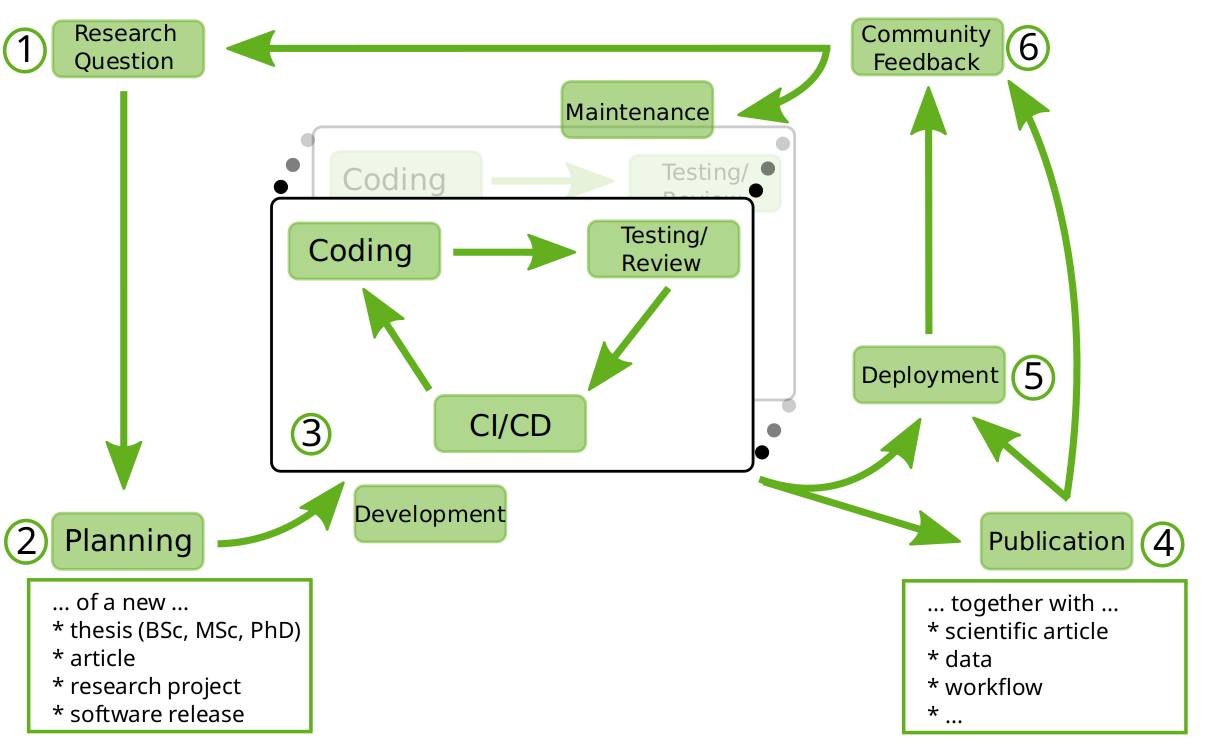
\includegraphics[width=0.99\linewidth]{imgs/rs_lifecycle.png}
    \caption{Research Software lifecycle.}
    \label{fig:rslifecycle}
\end{figure}

\subsection{Example of tools, services and infrastructures to implement Quality Assurance for RS}

% \violaine{The idea is to refer to some search software of the different categories and show the similarities and differences with
% the analysis of the top to point out the possible lacks in the current service offer} 
